
\section{Results}
\label{sec:results}

To demonstrate the effectiveness of the nested iterative algorithm, we utilize both analytical closed form functionals and scientific datasets in both 1-D and 2-D obtained from high-fidelity simulations. A brief description of the problem cases that are used as test datasets are given below.

\begin{enumerate}
	\item Synthetic data: sinc($x$)=$\frac{sin(x)}{x}$ functional on $\Omega \in [-4, 4]$
	\begin{itemize}
		\item 1-D: Q = (sinc($x$) + sinc(2*$x$-1) + sinc(3*$x$+1.5)), 
		\item 2-D: Q = (sinc($\sqrt{x^2+y^2}$))
	\end{itemize}
	\item Nek5000: A 3-D dataset from CFD simulation with velocity magnitude as the solution profile
	\item S3D: This is a 3-D turbulent combustion dataset generated by an S3D simulation \cite{chen-s3d-2009} of fuel jet combustion in the presence of an external cross-flow. 
	\item CESM: A 2-D Community Atmosphere Model climate model dataset on a sphere with 3600x1800 resolution
\end{enumerate}


\subsection{1-D Results}\label{AA}

%\begin{itemize}
%	\item Use the first two problems to measure convergence in parallel as number of domains increase
%	\item Talk about adaptivity and resolution of data even for highly varying problem data.
%\end{itemize}

\subsubsection{Adaptive Error Convergence and Verification}

The 1-D implementation of the ASM iterative solver was applied to the sinc problem. An initial input problem size of 500 points was evaluated as a test case, and MFA representation for the resulting profile was computed on 4 subdomains. The solution profile, along with the control point locations from the adaptive computation are shown in \fig{fig:sinc-adaptive-a}. We utilized the residual definition shown in \eqt{eq:nonlinear-residuals} with a $G_1$ constraint to be satisfied along all internal subdomain interfaces. The \fig{fig:sinc-adaptive-b} and \fig{fig:sinc-adaptive-c} present the zoomed in reconstruction of the approximation near the interface between $\Omega_2$ and $\Omega_3$ before, and after the ASM iterations are converged. The discontinuous representation of data when performing independent, adaptive, unconstrained subdomain solves are converged to satisfy the constraints after only 3 RAS iterations, with nearest neighbor exchange of control point data at the interfaces to recover $G_1$ continuity.

\begin{figure}
	\centering
	\subfloat[sinc function profile in 1-D\label{fig:sinc-adaptive-a}]{%
		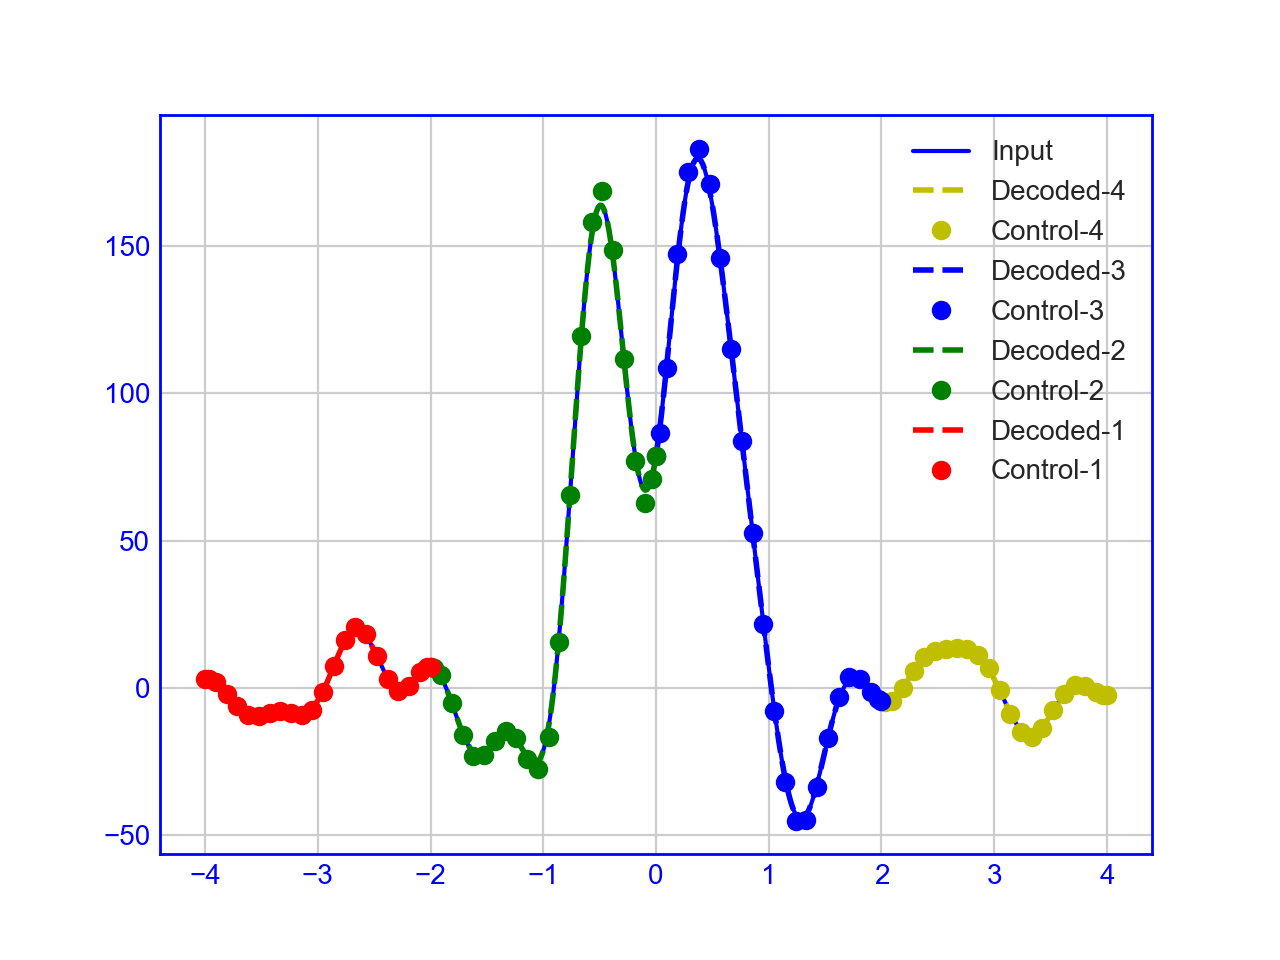
\includegraphics[width=0.5\textwidth]{figures/sinc-1d-profile}}
	\hfill
	\subfloat[Zoomed in image of $\Omega_{2,3}$ at (a) iASM=0\label{fig:sinc-adaptive-b}]{%
		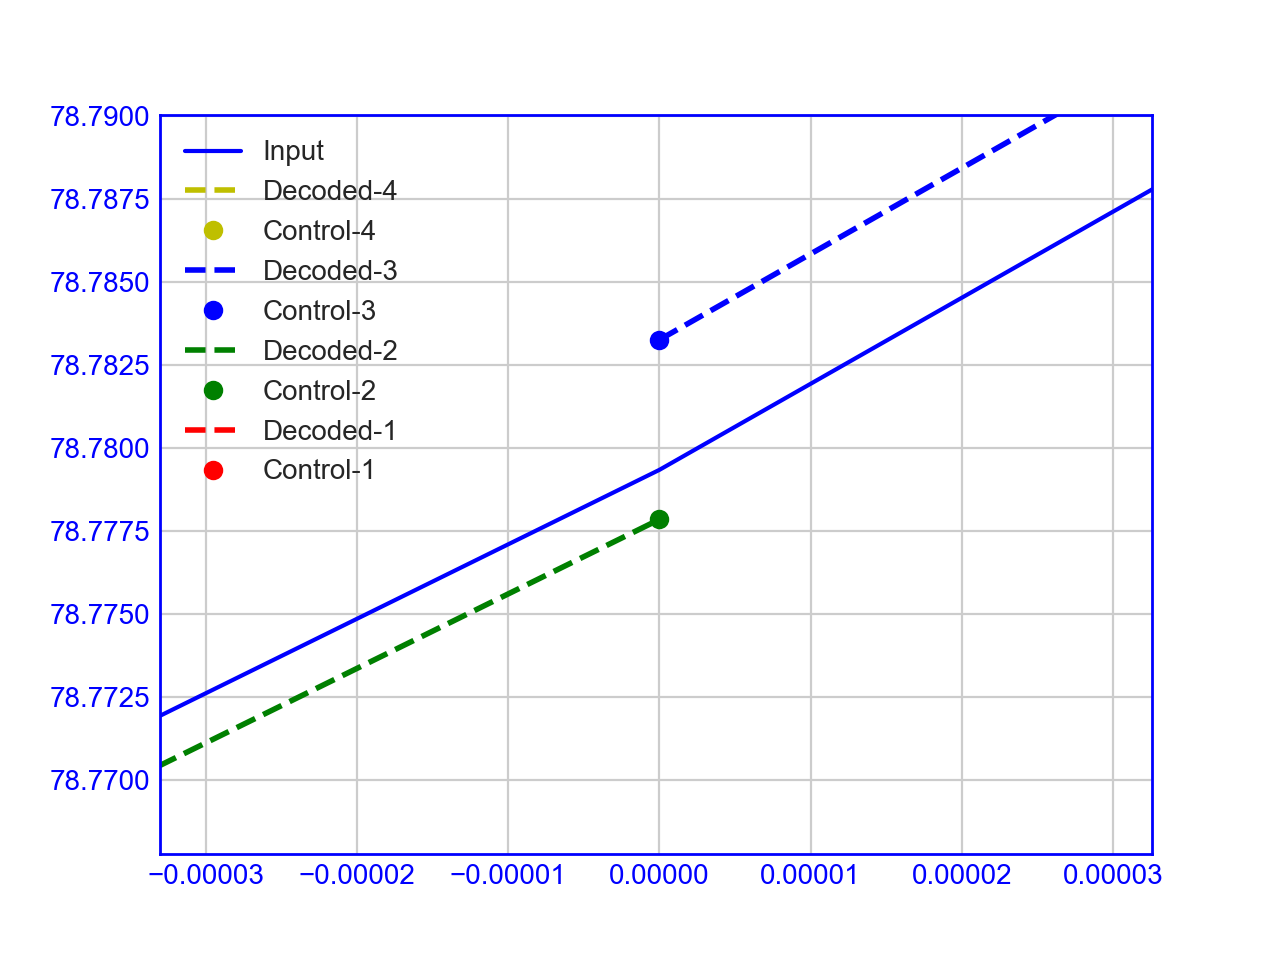
\includegraphics[width=0.5\textwidth]{figures/sinc-1d-discontinuous}}
	\\
	\subfloat[Zoomed in images of $\Omega_{2,3}$ at iASM=3\label{fig:sinc-adaptive-c}]{%
		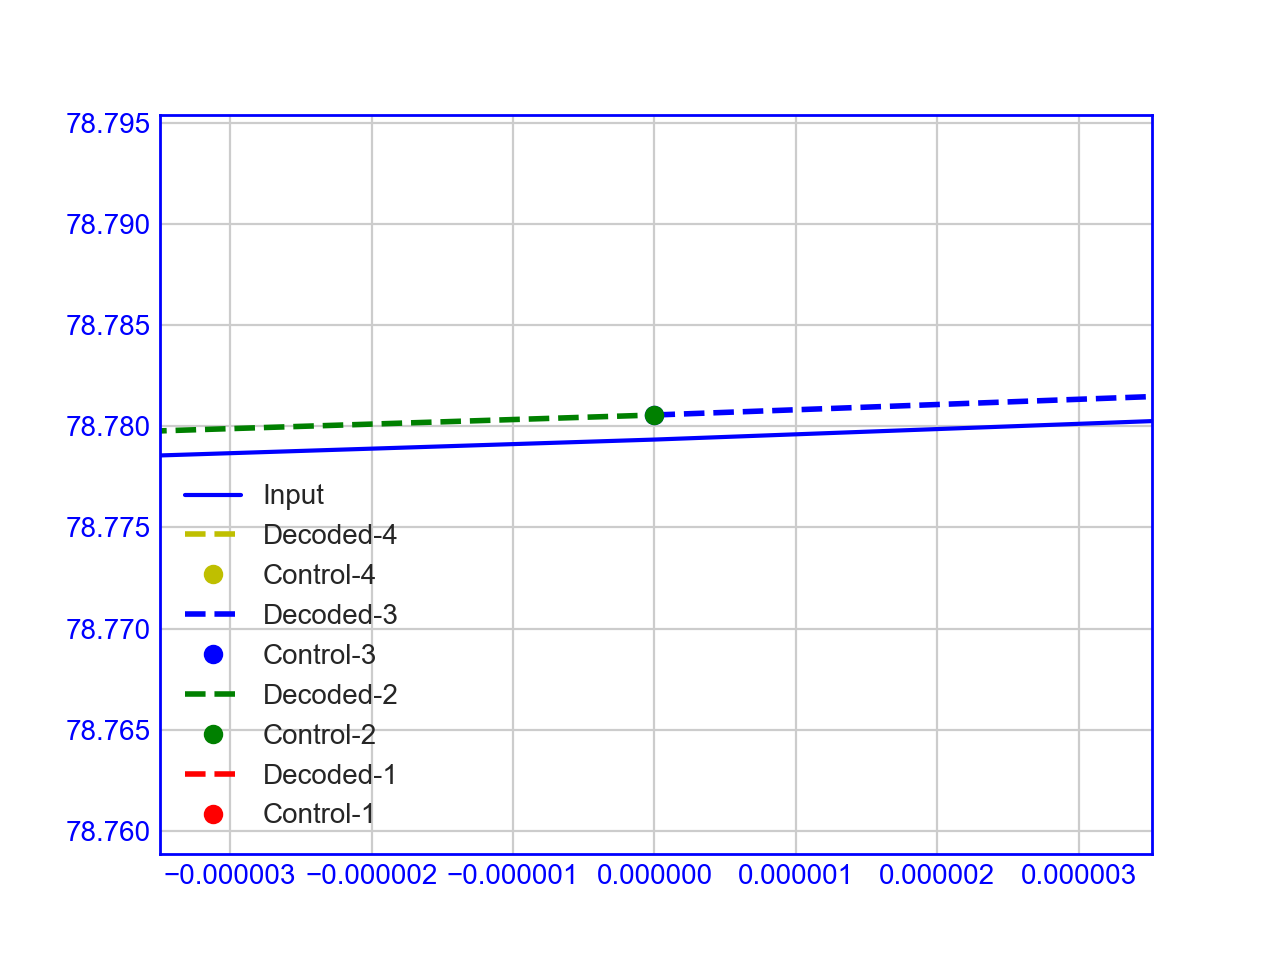
\includegraphics[width=0.5\textwidth]{figures/sinc-1d-continuous}}
	\caption{1-D analytical sinc dataset with 501 input points: adaptive MFA on 4 subdomains with $10^{-4}$ 	tolerance and $p=2$}
	\label{fig:sinc-adaptive}
\end{figure}

%\subsubsection{Subdomain Solver Performance}
%
%Compare LCLSQ - Encoded nonlinear and Decoded nonlinear

\subsubsection{Overlap Experiments in 1-D}

In this 1-D experiment on the closed form sinc function shown in \sect{sec:results}, we utilize the decoded residual minimization with the ASM-Krylov solver combination, and increase the amount of overlap in the input points to look at convergence speed. We measured the global $L_2$ error convergence along with the total cost in terms of outer iteration to compute the constrained control point locations. In this analysis, adaptivity in the individual subdomains was explicitly turned off so as to maintain a constant ratio of input points to control points per subdomain, as overlap region is extended in the subdomains on both the left and right sides.

\fig{fig:decoded-overlap-data-performance} shows the global $L_2$ norm of the net error in the decoded residual, as the number of subdomains are increased. With no overlap regions, where only the interface data is shared, the total ASM iterations needed to satisfy convergence, and the net error increase monotonically with $n_s$. As the overlap size becomes larger, for $\Delta=32$ and $\Delta=64$, the error growth and the iterations required remain much more bounded in comparison to the non-overlapping case. The implications of this particular result closely matches the DD ASM preconditioning theory often applied in PDE solvers \cite{smith-ddm, lions-asm, gander-rasm}. It also shows that the RAS iterative scheme can be accelerated more efficiently, and scalably used as a solver without a prohibitive linear complexity of O($n_s$).

\begin{figure}
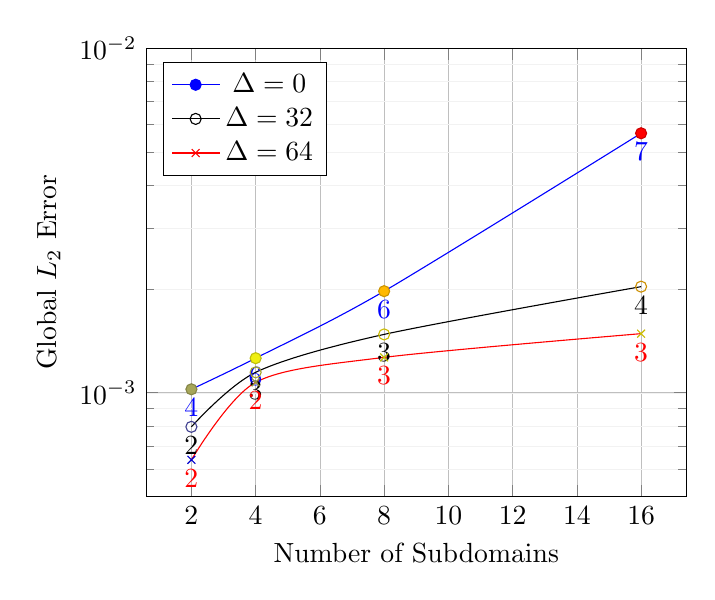
\begin{tikzpicture}

\begin{semilogyaxis}[
legend pos= north west,
ymin = 0.0005, ymax = 0.01,
xlabel=Number of Subdomains,
ylabel=Global $L_2$ Error,
nodes near coords*={\Label},
visualization depends on={value \thisrow{label} \as \Label},
grid=both,
grid style={line width=.1pt, draw=gray!10},
major grid style={line width=.2pt,draw=gray!50},
axis line style={latex-latex},
%axis lines=middle,
]
\axispath\draw
(7.49165,-10.02171)
|-  (8.31801,-11.32467)
node[near start,left] {$\frac{dy}{dx} = -2.58$};

\addplot[smooth,mark=*,blue] table [meta=class]  {
	x y class label
	2    0.001023481 A 4
	4    0.001259901 B 6
	8    0.001971792 C 6
	16   0.005663382 D 7
};

\addplot[smooth,mark=o,black] table [meta=class]  {
	x y class label
	2    0.000796565 A 2
	4    0.001146259 B 3
	8    0.001477074 C 3
	16   0.002032123 D 4
};

\addplot[smooth,mark=x,red] table [meta=class]  {
	x y class label
	2    0.000638741 A 2
	4    0.001072061 B 2
	8    0.001266798 C 3
	16   0.001484362 D 3
};

%\addplot[smooth,mark=*,blue] plot coordinates {
%	(2,    0.001023481)
%	(4,    0.001259901)
%	(8,    0.001971792)
%	(16,   0.005663382)
%};

%\addplot[smooth,mark=o,black] plot coordinates {
%	(2,    0.000796565)
%	(4,    0.001146259)
%	(8,    0.001477074)
%	(16,   0.002032123)
%};

%\addplot[smooth,mark=x,red] plot coordinates {
%	(2,    0.000638741)
%	(4,    0.001072061)
%	(8,    0.001266798)
%	(16,   0.001484362)
%};

\legend{$\Delta=0$\\$\Delta=32$\\$\Delta=64$\\}

\end{semilogyaxis}
\end{tikzpicture}
\caption{1-D sinc problem with 1025 points: Accuracy convergence and number of iterations of ASM solver with overlap variations, as $n_s$ increases}
\label{fig:decoded-overlap-data-performance}
\end{figure}

\subsection{2-D Results}

We utilize the described 2-D problem datasets to better understand the convergence and parallel scalability of the proposed algorithms at scale. Demonstrations for the S3D, Nek5000 and Climate datasets are provided below.

\subsubsection{S3D dataset}
Using the varying fidelity of the real world data, and the ability to create complex closed form functionals within our Python implementation, the approach was verification for accuracy using uniform control point refinements to yield sizes theoretical convergence orders. Additionally, using adaptive resolution based on a-posteriori gradient estimates, numerical errors in strongly varying solution profiles were reduced to within user-specified tolerances. A sample solution for the 2-D slice of the S3D dataset on 16 subdomains is shown in \fig{fig:s3d-adaptive-2d}.

\begin{figure}
	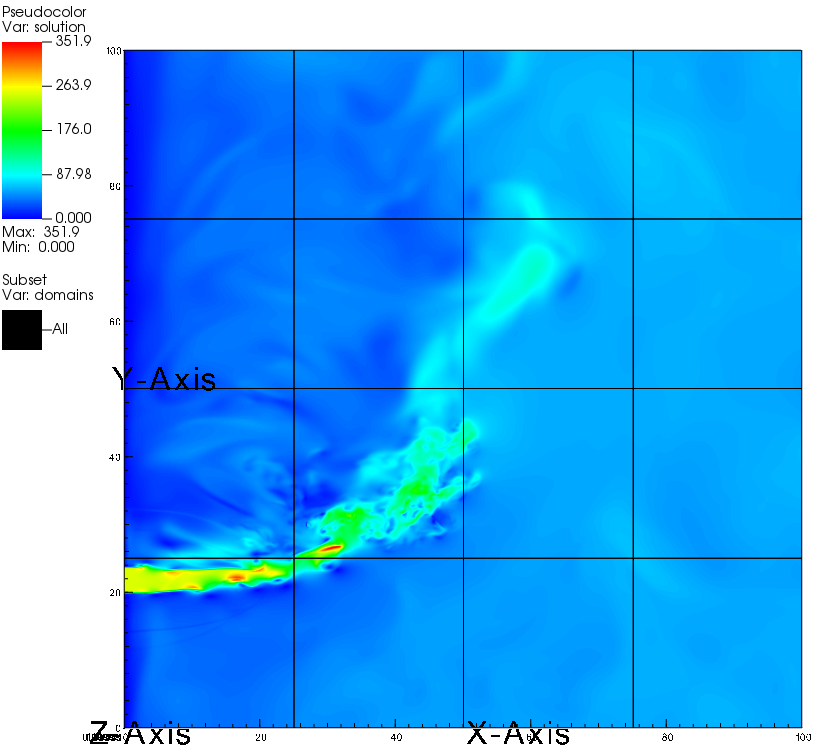
\includegraphics[width=0.45\textwidth]{figures/s3d-2d-profile.png}
	\caption{2-D slice of S3D dataset}
	\label{fig:s3d-adaptive-2d}
\end{figure}

\Remark{show error convergence plots for S3D on 16 subdomains with adaptivity}

\subsubsection{Nek5000 dataset}

\Remark{add table of actual compression and error as $n_s$ is changed}

\Remark{Discuss about complications and potential ways to enforce continuity. (a) Use decoded data, (b) Use control point space across interface}


\subsection{Parallel Scalability}\label{sec:parallel-scalability}

The parallel scalability of the implemented RAS iterative solver for ensuring continuity across block boundaries was measured on the 2-D CESM dataset, whose solution profile in a uniform latitude-longitude grid is shown in \fig{fig:cesm-2d-profile}. 
Our experiments were executed on the Bebop cluster at
Argonne National Laboratory LCRC (Laboratory Computing Resource Center). Bebop has 1024 public nodes, with Intel Broadwell or Intel Knights Landing processors, with 128 GB memory per Broadwell node, and 104 GB per KNL node. It has an Omni-Path Fabric Interconnect. Broadwell processors have 36 cores, while KNL processors have 64 cores. We primarily used the KNL processors for the scalability tests presented below.

A strong scalability test was performed on the Bebop cluster with the climate dataset, using 32 subdomains in X-direction and 128 subdomains in Y-direction. With this fixed DD and 100 control point per subdomain resolution, the driver utilized DIY to handle the block assignment to processes. As the total number of processes used in the parallel run was varied from [1,2,$\ldots$4096], we measured the overall time for the initial subdomain solves, and the consequent RAS iteration cycle for $nMaxASM=5$. The time to compute the MFA in parallel is shown for this strong scalability experiement in \fig{fig:cesm-strong-scalability}.

\begin{figure}
	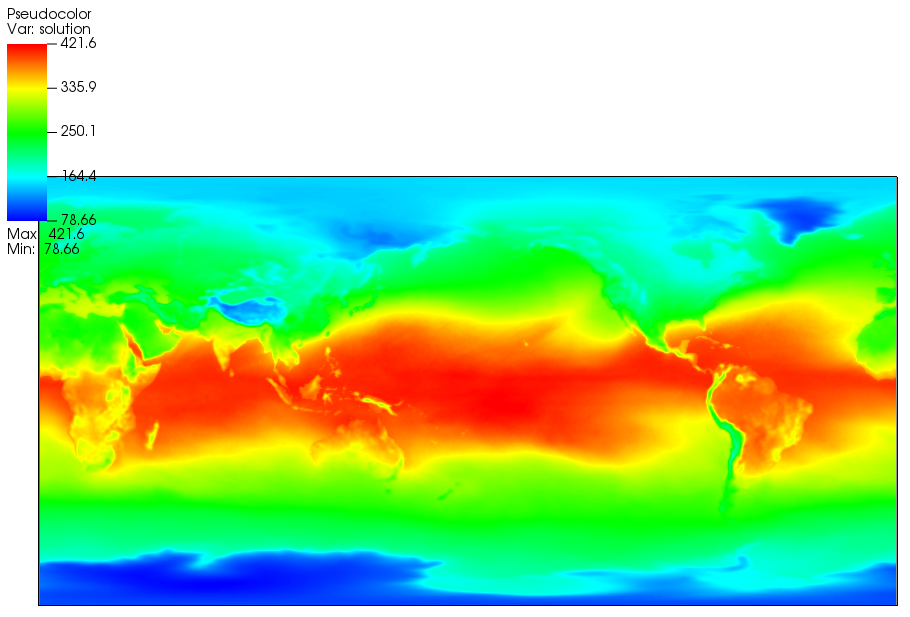
\includegraphics[width=0.45\textwidth]{figures/cesm-profile.png}
	\caption{2-D CESM climate dataset}
	\label{fig:cesm-2d-profile]}
\end{figure}

As expected, the hierarchical iterative scheme with RAS-Krylov combination shows excellent scalability for the chosen dataset and the overall time to compute the MFA was reduced from nearly 7000s on a single process,  to 9.5s on 2048 processes, while ensuring $G_0, G_1$ continuity in the domain interfaces. The ratio of computational work in local subdomain solves in comparison to communication time in nearest-neighbor exchanges gradually increases as subdomain size shrinks. This is due to the fact that global information on smaller subdomains take multiple iterations to propagate, and hence using overlaps for such large problems would be a recommended extension in the future to improve overall scalability of the algorithm.

%CESM dataset has 6.5M data points
%We used 32*128 = 4096 subdomains for the strong scaling test
%\Remark{How does the nearest neighbor communication stay bounded ? measure timings separately ?}

%jobrun_neup cesm_p1 1 1 python ../Projection-2D.py -x 32 -y 128 -p 5 -c 10 -a 5 --disableadaptivity 

\begin{figure}
	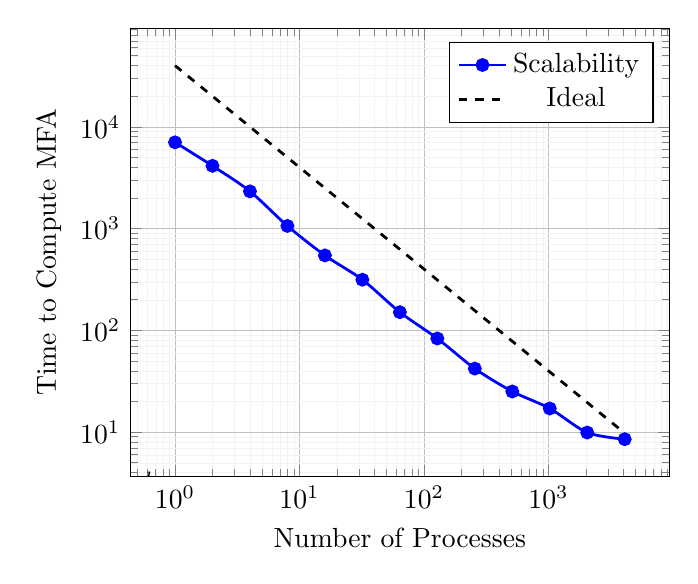
\begin{tikzpicture}
	
	\begin{loglogaxis}[
	legend pos= north east,
%	ymin = 0.0005, ymax = 0.01,
	xlabel=Number of Processes,
	ylabel=Time to Compute MFA,
%	nodes near coords*={\Label},
%	visualization depends on={value \thisrow{label} \as \Label},
	grid=both,
	grid style={line width=.1pt, draw=gray!10},
	major grid style={line width=.2pt,draw=gray!50},
	axis line style={latex-latex},
	every axis plot/.append style={line width=1.0pt},
	%axis lines=middle,
	]
	\axispath\draw
	(7.49165,-10.02171)
	|-  (8.31801,-11.32467)
	node[near start,left] {$\frac{dy}{dx} = -2.58$};
	
	\addplot[smooth,mark=*,blue,width=5pt] table [meta=eff]  {
		x y eff
		1	7045.451504	100
		2	4137.296798	85.14558959
		4	2322.884537	75.82653583
		8	1061.974002	82.92871918
		16	544.925238	80.80754722
		32	314.578249	69.98906001
		64	150.8316872	72.98544611
		128	83.16858159	66.18195096
		256	42.09792775	65.37446476
		512	25.07828297	54.870772
		1024	17.07229925	40.30109616
		2048	9.898160849	34.75556641
		4096	8.519652482	20.18956686
	};

	\addplot[dashed,black,width=2pt] table [meta=class]  {
	x y class 
	1	40000	100
	2	20000	100
	4	10000	100
	8	5000	100
	16	2500	100
	32	1250	100
	64	625	100
	128	312.5	100
	256	156.25	100
	512	78.125	100
	1024	39.0625	100
	2048	19.53125	100
	4096	9.765625	100
};
	
	\legend{Scalability\\Ideal\\}
	
	\end{loglogaxis}
	\end{tikzpicture}
	\caption{Strong Scalability of the 2-D CESM Problem with 4096 subdomains and 100 control points/subdomain}
	\label{fig:cesm-strong-scalability}
\end{figure}


%\paragraph{Positioning Figures and Tables} Place figures and tables at the top and 
%``Fig.~\ref{fig}'', even at the beginning of a sentence.

%\begin{table}[htbp]
%\caption{Table Type Styles}
%\begin{center}
%\begin{tabular}{|c|c|c|c|}
%\hline
%\textbf{Table}&\multicolumn{3}{|c|}{\textbf{Table Column Head}} \\
%\cline{2-4} 
%\textbf{Head} & \textbf{\textit{Table column subhead}}& \textbf{\textit{Subhead}}& \textbf{\textit{Subhead}} \\
%\hline
%copy& More table copy$^{\mathrm{a}}$& &  \\
%\hline
%\multicolumn{4}{l}{$^{\mathrm{a}}$Sample of a Table footnote.}
%\end{tabular}
%\label{tab1}
%\end{center}
%\end{table}

%\begin{figure}[htbp]
%\centerline{\includegraphics{fig1.png}}
%\caption{Example of a figure caption.}
%\label{fig}
%\end{figure}
